\section{Agent Evaluation and Benchmarking}

\begin{frame}{}
    \LARGE Agentic Models: \textbf{Evaluation and Benchmarking}

    \vspace{1em}
    \normalsize A leaderboard says 80\%. Eighty percent of what, measured how, and how many times?
\end{frame}

\begin{frame}{The Benchmark Lifecycle: Saturate, Audit, Replace}
    \begin{center}
    \small
    \renewcommand{\arraystretch}{1.2}
    \begin{adjustbox}{max width=\linewidth}\begin{tabular}{>{\raggedright\arraybackslash}p{2.5cm}>{\raggedright\arraybackslash}p{3.6cm}>{\raggedright\arraybackslash}p{3.4cm}>{\raggedright\arraybackslash}p{3.5cm}}
        \toprule
        \textbf{Family} & \textbf{First wave} & \textbf{Now} & \textbf{Successor} \\
        \midrule
        SWE-bench Verified & SWE-agent 12.5\% on the original (2024) & above 80\% (2026) & SWE-Bench Pro: best 61.5\% $\pm$3.1 \\
        OSWorld & best model 12.24\% (2024) & Verified: 60.76\% (2025) & OSWorld 2.0: best 20.6\% \\
        GAIA & GPT-4 with plugins 15\%, humans 92\% & 76.4\% (2025). The board looks inactive & \\
        BrowseComp & GPT-4o with browsing 1.9\% & 86.8\% with a multi-agent harness & \\
        $\tau$-bench & gpt-4o retail 61.2 & classic domains 80 to 92 & banking domain: 48.7 \\
        \bottomrule
    \end{tabular}\end{adjustbox}
    \end{center}
    \begin{itemize}\itemsep0.35em
        \item A benchmark's useful life is about \textbf{12 to 18 months} (our estimate). Day 2 covered reasoning benchmarks. These measure \emph{acting}.
    \end{itemize}
    \src{Deng et al., ``SWE-Bench Pro,'' \href{https://arxiv.org/abs/2509.16941}{arXiv:2509.16941}, and leaderboard (Oct 2026). Yuan et al., \href{https://arxiv.org/abs/2606.29537}{arXiv:2606.29537}. Mialon et al., ``GAIA,'' \href{https://arxiv.org/abs/2311.12983}{arXiv:2311.12983}. Wei et al., ``BrowseComp,'' \href{https://arxiv.org/abs/2504.12516}{arXiv:2504.12516}. Anthropic, Opus 4.6 announcement. $\tau^2$-bench leaderboard.}
\end{frame}

\begin{frame}{Anatomy of a Modern Agent Task}
    \begin{columns}[T,onlytextwidth]
        \column{0.5\textwidth}
        \begin{itemize}\itemsep0.45em
            \item \textbf{A Terminal-Bench 2.0 task} is an instruction, a Docker image, tests and an oracle solution. Tests look only at the \emph{final container state}.
            \item \textbf{Three properties to verify:}
            \begin{itemize}\itemsep0.15em
                \item \emph{Specificity}: tests pass if and only if the outcome is acceptable
                \item \emph{Solvability}: the oracle passes
                \item \emph{Integrity}: no shortcuts exist
            \end{itemize}
            \item About \textbf{3 reviewer-hours per task}. 89 tasks kept out of 229 contributed.
        \end{itemize}
        \column{0.48\textwidth}
        \centering
        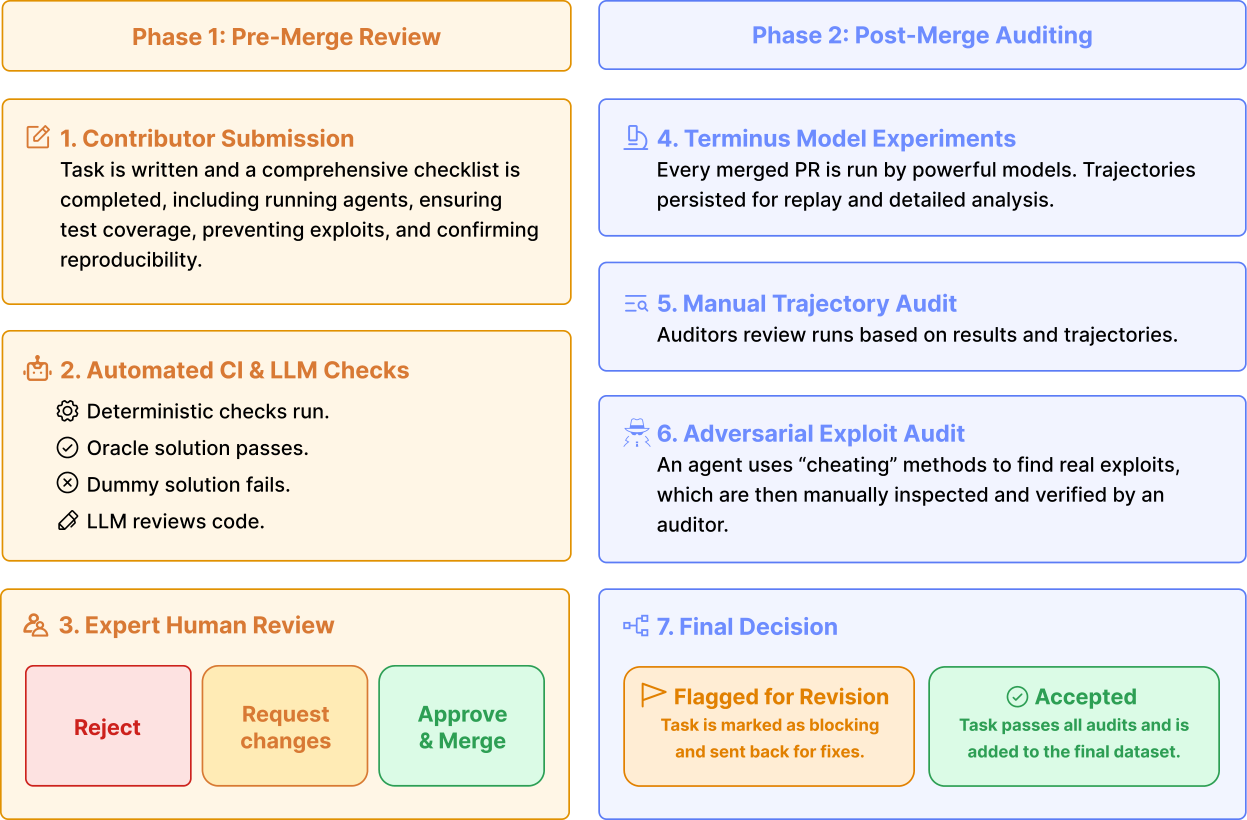
\includegraphics[width=\linewidth,height=0.62\textheight,keepaspectratio]{images/agentic-models-memory/tbench_review_process.png}
    \end{columns}
    \vspace{0.2em}
    \takeaway{Building a trustworthy agent benchmark is now \textbf{security engineering}: assume the agent will find any shortcut you left.}
    \src{Merrill et al., ``Terminal-Bench,'' \href{https://arxiv.org/abs/2601.11868}{arXiv:2601.11868}, Figures 2 and 3.}
\end{frame}

\begin{frame}{Time Horizons: Measuring Autonomy in Human Hours}
    \begin{columns}[T,onlytextwidth]
        \column{0.6\textwidth}
        \centering
        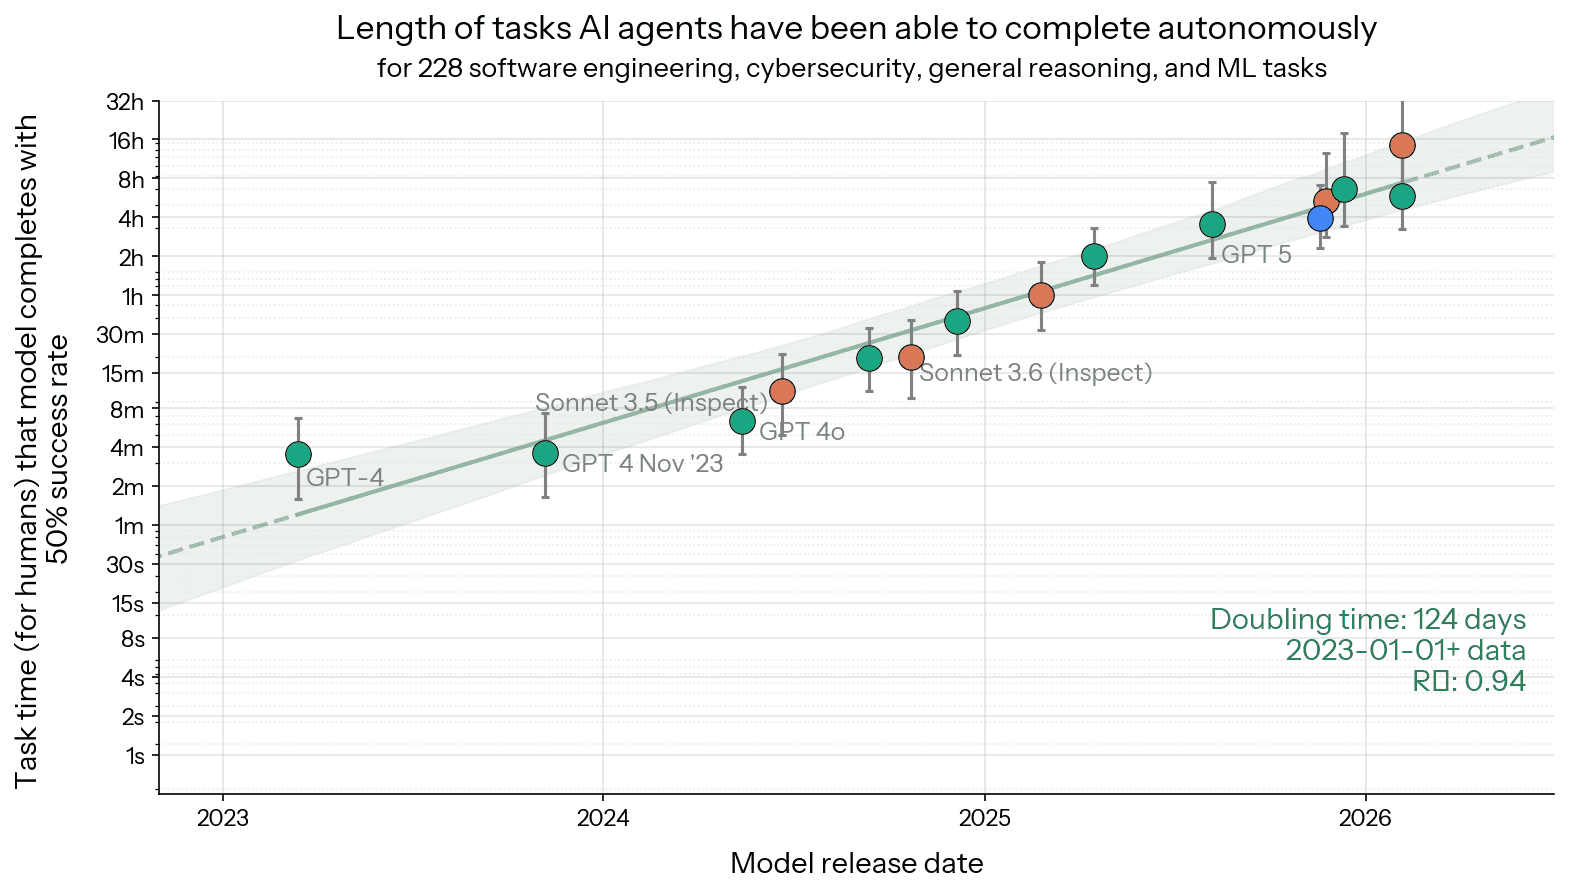
\includegraphics[width=\linewidth,height=0.55\textheight,keepaspectratio]{images/agentic-models-memory/metr_length_of_tasks_log.png}
        \column{0.38\textwidth}
        \centering
        \footnotesize
        \renewcommand{\arraystretch}{1.15}
        \begin{adjustbox}{max width=\linewidth}\begin{tabular}{lrr}
            \toprule
            \textbf{Horizon (min)} & \textbf{50\%} & \textbf{80\%} \\
            \midrule
            Claude 3.7 Sonnet & 60 & 12 \\
            GPT-5 & 203 & 38 \\
            Claude Opus 4.5 & 293 & 49 \\
            Gemini 3.1 Pro & 384 & 90 \\
            Claude Opus 4.6 & 719 & 70 \\
            Mythos Preview & 1,045 & 186 \\
            \bottomrule
        \end{tabular}\end{adjustbox}
    \end{columns}
    \vspace{0.2em}
    \begin{itemize}\itemsep0.3em
        \item \textbf{Method.} Time human experts per task, fit model success against log task length, read off the 50\% (or 80\%) crossing.
        \item \alert{Read the intervals.} Opus 4.6's 50\% horizon has a confidence interval of 317 to 3,634 minutes.
    \end{itemize}
    \src{Kwa et al., ``Measuring AI Ability to Complete Long Software Tasks,'' \href{https://arxiv.org/abs/2503.14499}{arXiv:2503.14499}. Figure: METR, live chart (its fitted doubling time differs slightly from the table's source). Table: METR time-horizons data, updated 8 May 2026.}
\end{frame}

\begin{frame}{The Harness Is Part of the Score}
    \begin{center}
    \small
    \renewcommand{\arraystretch}{1.2}
    \begin{adjustbox}{max width=\linewidth}\begin{tabular}{>{\raggedright\arraybackslash}p{2.6cm}>{\raggedright\arraybackslash}p{7.4cm}>{\raggedright\arraybackslash}p{2.8cm}}
        \toprule
        \textbf{Model} & \textbf{Terminal-Bench 2.0 score by harness} & \textbf{Spread} \\
        \midrule
        GPT-5 & Codex CLI 49.6, OpenHands 41.5, Terminus 2 35.2, Mini-SWE-Agent 33.9 & 15.7 points \\
        Claude Opus 4.5 & Terminus 2 57.8, Claude Code 52.1, OpenHands 51.9 & 5.9 points \\
        Gemini 2.5 Pro & Terminus 2 32.6, Mini-SWE-Agent 26.1, Gemini CLI 19.6, OpenHands 15.7 & \alert{2.1$\times$} \\
        \bottomrule
    \end{tabular}\end{adjustbox}
    \end{center}
    \begin{itemize}\itemsep0.4em
        \item \textbf{Tokens vary even more.} Opus 4.5 used 3.9M input tokens on one harness and 256.9M on another.
        \item \textbf{Leaderboard ranks are often ties.} SWE-Bench Pro intervals are about $\pm$3.6 points, and five models share rank 5.
    \end{itemize}
    \takeaway{A score is a tuple: model, scaffold, budget, trials, task subset, grader version, confidence interval.}
    \src{Merrill et al., \href{https://arxiv.org/abs/2601.11868}{arXiv:2601.11868}, Table 2. Scale AI, SWE-Bench Pro public leaderboard (Oct 2026).}
\end{frame}

\begin{frame}{Cost and Reliability Are First-Class Axes}
    \begin{columns}[T,onlytextwidth]
        \column{0.5\textwidth}
        \textbf{Cost}
        \begin{itemize}\itemsep0.4em
            \item HAL's summary: agents ``can be 100x more expensive while only being 1\% better''.
            \item In \textbf{21 of 36} model, agent and benchmark combinations, more reasoning effort gave equal or \emph{lower} accuracy.
        \end{itemize}
        \column{0.48\textwidth}
        \textbf{Reliability}
        \begin{itemize}\itemsep0.4em
            \item Over 24 months, accuracy climbed while reliability improved only slightly.
            \item Agents tolerate infrastructure faults but \alert{break under paraphrase} of the task.
        \end{itemize}
    \end{columns}
    \vspace{0.5em}
    \begin{center}
    \small
    \begin{adjustbox}{max width=\linewidth}\begin{tabular}{>{\raggedright\arraybackslash}p{2.6cm}>{\raggedright\arraybackslash}p{10.2cm}}
        \toprule
        \textbf{Dimension} & \textbf{Reliability metrics (12 in total)} \\
        \midrule
        Consistency & same outcome, same trajectory, same resource use across runs \\
        Robustness & fault injection, environment perturbation, paraphrase \\
        Predictability & calibration, discrimination, Brier score \\
        Safety & compliance, harm severity \\
        \bottomrule
    \end{tabular}\end{adjustbox}
    \end{center}
    \src{Kapoor et al., ``Holistic Agent Leaderboard,'' \href{https://arxiv.org/abs/2510.11977}{arXiv:2510.11977}. Rabanser et al., ``Towards a Science of AI Agent Reliability,'' \href{https://arxiv.org/abs/2602.16666}{arXiv:2602.16666}.}
\end{frame}

\begin{frame}{Broken Benchmarks, Quantified}
    \begin{center}
    \small
    \renewcommand{\arraystretch}{1.2}
    \begin{adjustbox}{max width=\linewidth}\begin{tabular}{>{\raggedright\arraybackslash}p{2.9cm}>{\raggedright\arraybackslash}p{6.1cm}>{\raggedright\arraybackslash}p{3.8cm}}
        \toprule
        \textbf{Benchmark} & \textbf{Flaw} & \textbf{Effect} \\
        \midrule
        $\tau$-bench & an empty response counts as success on impossible tasks & 38\% overestimate \\
        SWE-bench Verified & insufficient tests & 24\% of top-50 ranks change \\
        SWE-Lancer & the agent can read the test files & 100\% without solving anything \\
        OSWorld & selectors broke when websites changed & 28\% \emph{under}estimate \\
        \bottomrule
    \end{tabular}\end{adjustbox}
    \end{center}
    \begin{itemize}\itemsep0.35em
        \item Of 10 benchmarks audited, 7 violate \textbf{task validity} (solvable if and only if the agent has the skill) and 7 violate \textbf{outcome validity} (a pass means success).
        \item Google found 3 SWE-bench Verified items that \emph{no solution can pass}.
    \end{itemize}
    \src{Zhu et al., ``Establishing Best Practices for Building Rigorous Agentic Benchmarks,'' \href{https://arxiv.org/abs/2507.02825}{arXiv:2507.02825}. Google DeepMind, Gemini 3.1 Pro Model Evaluation.}
\end{frame}

\begin{frame}{Passing Tests Is Not Finished Work}
    \begin{columns}[T,onlytextwidth]
        \column{0.44\textwidth}
        \centering
        \begin{adjustbox}{max width=\linewidth}\begin{tikzpicture}
            \begin{axis}[
                ybar, bar width=16pt, width=6.4cm, height=4.7cm,
                ymin=0, ymax=50, ylabel={\% of pull requests},
                symbolic x coords={Pass tests,Mergeable as-is},
                xtick=data, x tick label style={font=\scriptsize},
                y label style={font=\scriptsize}, y tick label style={font=\scriptsize},
                nodes near coords, nodes near coords style={font=\scriptsize},
                axis lines*=left, ymajorgrids, grid style={gray!20}, enlarge x limits=0.6]
                \addplot[fill=KAred!45, draw=KAred!75!black] coordinates {(Pass tests,38) (Mergeable as-is,0)};
            \end{axis}
        \end{tikzpicture}\end{adjustbox}

        {\scriptsize Claude 3.7 Sonnet on real repository tasks, judged by maintainers (METR, small sample).}
        \column{0.54\textwidth}
        \begin{itemize}\itemsep0.45em
            \item Every test-passing pull request still lacked adequate tests. Most had documentation and lint gaps.
            \item \textbf{For your own agent, use three graders:}
            \begin{itemize}\itemsep0.15em
                \item \emph{code-based}: fast and reproducible, but brittle
                \item \emph{model-based}: flexible, but non-deterministic
                \item \emph{human}: the gold standard, but slow
            \end{itemize}
            \item \textbf{Validate the judge.} A trajectory judge reached 90\% agreement with humans on 120 labelled traces. Elsewhere, no single LLM judge was best on every benchmark.
            \item Start from 20 to 50 real failures. Move saturated evaluations into a regression suite.
        \end{itemize}
    \end{columns}
    \vspace{0.2em}
    \src{Rein, ``Research update: towards reconciling slowdown with time horizons'' (METR, Aug 2025). Grace et al., ``Demystifying evals for AI agents'' (Anthropic, Jan 2026). Merrill et al., \href{https://arxiv.org/abs/2601.11868}{arXiv:2601.11868}. L\`u et al., ``AgentRewardBench,'' \href{https://arxiv.org/abs/2504.08942}{arXiv:2504.08942}.}
\end{frame}

\begin{frame}{Evaluation: What to Remember}
    \begin{itemize}\itemsep0.6em
        \item First-generation agent benchmarks are \textbf{saturated or replaced}. Check the date and the version of any number.
        \item An agent score is a property of the whole stack: \textbf{model, scaffold, environment and grader}.
        \item \textbf{Time horizons} turn success rates into human task length. The gap between the 50\% and 80\% horizons is the reliability lesson.
        \item Many benchmarks are \textbf{broken in measurable ways}. Ask about task validity and outcome validity.
        \item Passing tests, low cost and consistent behaviour are three different things. Measure each.
    \end{itemize}
    \vspace{0.4em}
    \takeaway{\textbf{Next.} An agent that works 12 hours unattended, with tools, memory and peers, is a production system. How do we operate it safely?}
\end{frame}
